% Created 2022-04-09 sam. 15:57
% Intended LaTeX compiler: pdflatex
\documentclass[11pt]{article}
\usepackage[utf8]{inputenc}
\usepackage[T1]{fontenc}
\usepackage{graphicx}
\usepackage{grffile}
\usepackage{longtable}
\usepackage{wrapfig}
\usepackage{rotating}
\usepackage[normalem]{ulem}
\usepackage{amsmath}
\usepackage{textcomp}
\usepackage{amssymb}
\usepackage{capt-of}
\usepackage{hyperref}
\usepackage{lmodern} % Ensures we have the right font
\usepackage{graphicx}
\usepackage{amsmath, amsthm, amssymb}
\usepackage[table, xcdraw]{xcolor}
\usepackage{fancyhdr}
\usepackage[left=2cm,right=2cm,top=3cm,bottom=3cm]{geometry}
\pagestyle{fancy}
\fancyhf{}
\lhead{Modify in current org file : \lhead{foo}}
\rfoot{Page \thepage}
\usepackage{titling}
\setlength{\droptitle}{-8ex}
\pretitle{\begin{flushleft}\Large\bfseries}
\posttitle{\par\end{flushleft}}
\preauthor{\begin{flushleft}\large}
\postauthor{\end{flushleft}}
\predate{\begin{flushleft}}
\postdate{\end{flushleft}}
\usepackage[normalem]{ulem}
\usepackage{sectsty}
\sectionfont{\underline}
\makeatletter
\def\@seccntformat#1{%
\expandafter\ifx\csname c@#1\endcsname\c@section\else
\csname the#1\endcsname\quad
\fi}
\makeatother
\definecolor{bblue}{HTML}{275382}
\usepackage[colorlinks]{hyperref}
\hypersetup{colorlinks, linkcolor=bblue, urlcolor=bblue}
\usepackage[font={color=gray},figurename=Fig.,labelfont={it}]{caption}
\setlength{\parindent}{0pt}
\usepackage{graphicx}
\setkeys{Gin}{width=0.8\linewidth}
\setkeys{Gin}{height=0.7\textheight}
\setkeys{Gin}{keepaspectratio}
\usepackage{enumitem}
\setlist{noitemsep}
\setlist[itemize]{noitemsep}
\renewcommand{\contentsname}{Sommaire}
\usepackage{listings}
\usepackage{xcolor}
\usepackage[utf8]{inputenc}
\usepackage[table]{color}
\definecolor{grayW}{rgb}{0.94,0.94,1.00}
\definecolor{bluegr}{rgb}{0.0,0.50,0.50}
\definecolor{redp}{rgb}{0.80,0.10,0.10}
\lstset{
backgroundcolor=\color{grayW},
keywordstyle=\color{bluegr},
stringstyle=\color{redp},
basicstyle=\ttfamily\scriptsize,
breakatwhitespace=false,
numbers=left,
numbersep=5pt,
}
\lhead{DUREL Enzo, VILLEPREUX Thibault}
\rhead{POO - Puissance 4}
\author{DUREL Enzo, VILLEPREUX Thibault}
\date{\today}
\title{Projet - Puissance 4 - Java}
\hypersetup{
 pdfauthor={DUREL Enzo, VILLEPREUX Thibault},
 pdftitle={Projet - Puissance 4 - Java},
 pdfkeywords={},
 pdfsubject={},
 pdfcreator={Emacs 27.1 (Org mode 9.3)}, 
 pdflang={English}}
\begin{document}

\maketitle
\tableofcontents

\thispagestyle{fancy}

\newpage

\section{Introduction}
\label{sec:org0d4356b}

\subsection{Compilation}
\label{sec:org0208f85}

Lancez le Makefile avec la commande \texttt{make} dans le dossier \texttt{cd projet-java}.

\subsection{Exécution}
\label{sec:org230b547}

Exécuter le script bash \textbf{exec} qui lance le programme \textbf{Main} dans le dossier
\textbf{projet-java/build}.

Si une erreur survient lors du programme, elle est écrite dans le fichier
\textbf{log.txt}. 

\subsection{Puissance 4}
\label{sec:org77dc623}

Le principe est simple : insérer un pion chacun son tour dans la grille
verticale. Le gagnant est le premier à avoir aligné 4 pions de la même
couleur, horizontalement, verticalement, ou en diagonale. Tout l'enjeu de la
partie réside dans la stratégie adoptée pour mettre l'adversaire en échec.

\newpage

\section{UML du Puissance 4}
\label{sec:orgd9aa359}

\begin{figure}[htbp]
\centering
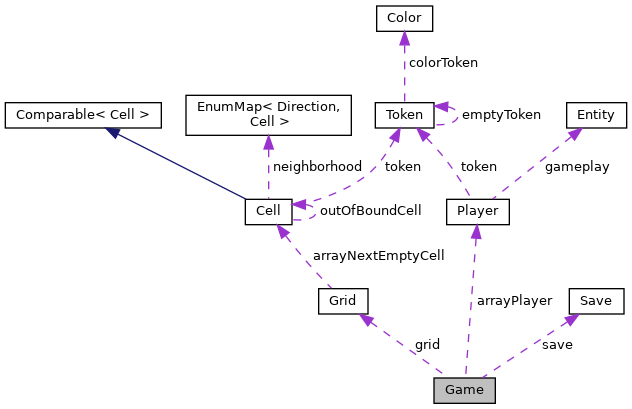
\includegraphics[width=.9\linewidth]{../doc/html/class_game__coll__graph.png}
\caption{UML du Puissance 4}
\end{figure}

\section{Explication de code}
\label{sec:org4440d4f}
\subsection{Introduction}
\label{sec:org61115cd}

La documentation étant entièrement disponible, nous allons nous attarder
uniquement sur les principales classes de notre logiciel ainsi que leur
fonctionnement global.\\

Pour cela nous nous appuirons sur le diagramme de la classe ainsi que
certaines fonctions jugées principales qui sont expliquées avec leurs \hyperref[org29fdec9]{graphes
respectifs}. 

\subsection{Classe Cell\label{org0ebae20}}
\label{sec:org05b22ae}

Nous allons maintenant présenter la classe qui représente une \textbf{case} du
plateau de jeu du puissance 4. Il s'agit de \texttt{public class Cell}.

\subsubsection{Attributs}
\label{sec:orgd8dea29}

Nous avons redéfini la cellule \texttt{null}, celle-ci s'appelle outOfBoundCell et
est renvoyé lorsque qu'on accès à une cellule qui n'existe pas. Nous avons
rédéfini car plus compréhensible sémantiquement et pour éviter d'avoir des
null qui se promène dans notre code. Cet attribut est statique donc
toujours de même référence.\\

Chaque cellule possède un jeton (Token) qui est ici juste un objet
possédant une certaine couleur (\hyperref[orgc449396]{Color}).\\

Chaque cellule possède aussi 4 voisins directes (\textbf{UP}, \textbf{DOWN}, \textbf{RIGHT},
\textbf{LEFT}) représenté ici par une EnumMap où les clés sont une direction
(\hyperref[org149a95e]{Direction}) donnée et les valeurs la référence à sa cellule voisine dans la
direction.\\

\subsubsection{Méthodes}
\label{sec:org969792b}

\begin{enumerate}
\item \texttt{setNeighbor: Cell*Direction -> ()} \label{org11ccfe8}
\label{sec:orge3e5f26}

Cette méthode prend en paramètre une cellule (\hyperref[org0ebae20]{Cell}) et une direction
(\hyperref[org149a95e]{Direction}) où la cellule représente la cellule voisine a attribue dans la
direction par rapport à la cellule dont la méthode est appelée.\\

Elle actualise l'EnumMap représentant les voisins d'une cellule dont la
clé est la direction donnée. La cellule doit être non \texttt{null}, la direction
doit être non \texttt{null}.\\

\item \texttt{getNeighbor: Direction -> Cell} \label{org7edf579}
\label{sec:org781b4c6}

Cette méthode prend en paramètre une direction (\hyperref[org149a95e]{Direction}) et renvoie la
cellule voisine dans la direction de la cellule qui appelle la méthode.\\

Dans le cas où la cellule voisine est null, la cellule invalide
outOfBoundCell est renvoyée. La direction doit être non nulle.\\

\item \texttt{check: () -> boolean}
\label{sec:orgbe5d63b}

La fonction check vérifie si la cellule qui appelle la méthode satisfait
les conditions d'arrêt du jeu: ici si 4 jeton (Token) de suite, sont de la
même couleur et aligné suivant la même direction.\\

Donc nous vérifions pour chaque direction possible acceptés si le nombre
dans la direction donnée de jetons de la même couleurs est supérieur ou
égal à 4.\\

Pour cela nous utilisons deux méhodes définies en surcharges.\\

La première ne prend en paramètre qu'une seule direction et compte suivant
les directions des cellules voisines directes (\textbf{UP}, \textbf{DOWN}, \textbf{RIGHT},
\textbf{LEFT})\\

La deuxième prend en paramètre deux directions qui définiront le comptage
en diagonale. En effet, une diagonale n'est juste composé de 2 directions
primitives.\\

Les diagonales sont récupérées dans l'Enum (\hyperref[org149a95e]{Direction}) par la méthode
\texttt{getDiagonales} et sont renvoyé sous la forme d'une EnumMap où les clés
sont les directions primitives et les valeurs une direction associée
formant une diagonales. Les diagonales renvoyées sont uniques.\\

Le nombre de voisin est définit par la somme des même cellules à partir de
la cellule courante dans la direction donnée et dans sa direction opposé
qui est récupéré grâce à la fonction \texttt{getOpposite} dans l'Enum
(\hyperref[org149a95e]{Direction}).\\

\begin{figure}[htbp]
\centering
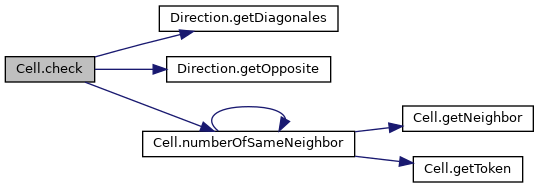
\includegraphics[width=10cm]{../doc/html/class_cell_ad03ad111fdf4eff6a3572deee55e0d1f_cgraph.png}
\caption{Graph d'appels de Cell.check()}
\end{figure}

\begin{enumerate}
\item \texttt{numberOfSameNeighbor: Direction -> int}
\label{sec:org0e3b6b6}

Cette méthode prend en paramètre une direction et compte dans cette
direction et à partir de la cellule le nombre de jetons similaires.\\

Elle utilise pour cela la récursivité. Le cas d'arrêt est : Si la
prochaine cellule est la cellule invale outOfBoundCell ou que le jeton de
la cellule n'est plus le même que la cellule précédente. Sinon, elle
renvoie 1 + appel de cette méthode sur la cellule suivant dans la
direction donnée.\\

\item \texttt{numberOfSameNeighbor: Direction*Direction -> int}
\label{sec:orge2dd661}

Cette méthode est similaire à la précédente, la prochaine cellule est la
cellule suivant les deux directions données. La condition d'arrêt est la
même, l'appel récursif est le même.\\
\end{enumerate}
\end{enumerate}

\subsection{Classe Grid\label{org8ee15bf}}
\label{sec:org5ca9b44}

Nous allons maintenant présenter la classe qui représente \textbf{le plateau de
jeu} du puissance 4. Il s'agit de \texttt{public class Grid}.\\

\subsubsection{Attributs}
\label{sec:org18fdbf3}

La classe \hyperref[org8ee15bf]{Grid} est composé d'un tableau de cellules (\hyperref[org0ebae20]{Cell}) contenant les
prochaines cellules vides de chaque colonnes. Lorsque la colonne est
pleine, la prochaine cellule vide est la cellule située la plus haute dans
la grille.\\

Nous avons utilisée cette représentation parce que sémantiquement nous
n'avions besoin que de savoir cela pour permettre au joueur de jouer. De
plus nous avons donc un gain de mémoire.\\

La classe comporte également deux attributs static représentant
respectivement la largeur \textbf{WIDTH} et la hauteur \textbf{HEIGHT}.\\

\subsubsection{Méthodes}
\label{sec:orgfe5522e}

Nous allons vous présenter maintenant quelques fonctions principales de
cette classe.\\

\begin{enumerate}
\item \texttt{initGrid: () -> ()}
\label{sec:orgcb28ef3}

Voici la fonction d'initialisation de la grille. Elle crée un tableau 2D
de cellules (\hyperref[org0ebae20]{Cell}), elle assigne à chaque cellule leurs voisins respectifs
(\textbf{UP}, \textbf{DOWN}, \textbf{RIGHT}, \textbf{LEFT}) grâce à la fonction \hyperref[org11ccfe8]{setNeighbor: Cell *
Direciton ->()} de (\hyperref[org0ebae20]{Cell}).\\

Nous remplissons ensuite le tableau des prochaines cellules vides définis
précédement en prenant comme première cellule la cellule situé la plus en
bas de chaque colonnes (car grille initialisé à vide).\\

\begin{figure}[htbp]
\centering
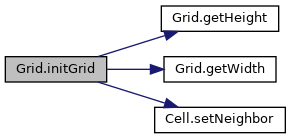
\includegraphics[width=5cm]{../doc/html/class_grid_a19c4d85a8586416e1b0dbcde22ef40ce_cgraph.png}
\caption{Graph d'appels de Grid.initGrid()}
\end{figure}

\item \texttt{getNextEmptyCellAt: int -> Cell}
\label{sec:org346831b}
Cette méthode permet de nous renvoyer la prochaine cellule à remplir pour
une colonne donnée en paramêtre.\\

C'est un accesseur utilisé lorsque l'on veut jouer un nouveau jeton.\\

Si la colonne est déjà remplie, elle nous renvoie la cellule spécifique
outOfBoundCell.\\

Elle vérifie quand même que la colonne existe, sinon elle renvoie une
IllegalArgumentException : "column outOfBound".\\

\begin{figure}[htbp]
\centering
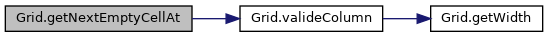
\includegraphics[width=10cm]{../doc/html/class_grid_afebd807863b80c631a1296ee320d09de_cgraph.png}
\caption{Graph d'appels de Grid.getNextEmptyCellAt()}
\end{figure}

\item \texttt{UpToNextEmptyCellAt: int -> ()}
\label{sec:org9eb5b4a}
Cette méthode permet de mettre à jour notre tableau de cellule
"arrayNextEmptyCell" avec comme indice le numéro de la colonne passé en
paramètre.\\

Elle regarde s'il existe une cellule en haut de la dernière colonne
pointée, c'est-à-dire une cellule différente de outOfBound.\\

Si c'est le cas, on change dans tableau la référence vers la prochaine
cellule.\\

Cette méthode fonctionne avec effet de bord.\\

\begin{figure}[htbp]
\centering
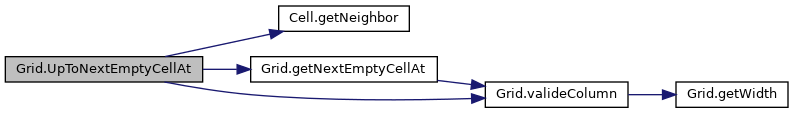
\includegraphics[width=.9\linewidth]{../doc/html/class_grid_a42995be492ec8858fcd8359538a2705c_cgraph.png}
\caption{Graph d'appels de Grid.UpToNextEmptyCellAt()}
\end{figure}

\item \texttt{loadGrid: String*Token[] -> ()}
\label{sec:orgcee8de1}
Cette méthode comme son nom l'indique, permet de charger la grille
précédemment lue dans un fichier.
Grâce à la lecture du fichier, nous obtenons un String et notre objectif
est alors de le transformer en Grid.\\

Pour cela on créé un tableau de cellules temporaires qui va contenir
toutes les cellues de la grille sous forme de String. Remplir ce tableau
se fait grâce à la fonction split(";").\\

Notre tableau commence par la cellule située en haut à gauche de la grille
et se termine par la cellule en bas à droite.\\

Puis pour chaque cellule, on récupère sa couleur et on l'enregistre dans
la grille.\\

\begin{figure}[htbp]
\centering
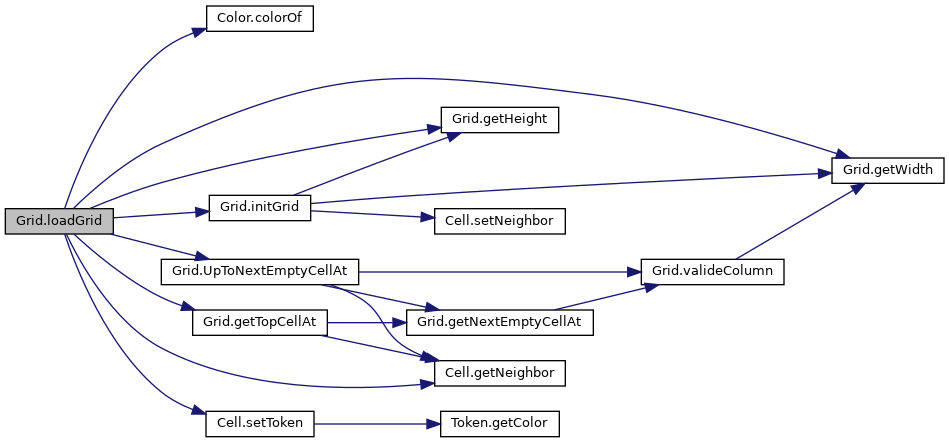
\includegraphics[width=.9\linewidth]{../doc/html/class_grid_ac5c22e855cdb16a15035f8f929ac90da_cgraph.png}
\caption{Graph d'appels de Grid.loadGrid()}
\end{figure}
\end{enumerate}

\subsection{Classe Player\label{orgfd9bf3b}}
\label{sec:org19348e7}
\subsubsection{Attributs}
\label{sec:org436f875}

La classe comporte trois attributs :
\begin{itemize}
\item Le pseudo du joueur: String
\item Le jeton du joueur: Token
\item La nature du joueur: Entity (LOCAL ou IA)
\end{itemize}

Remarquons qu'un joueur est défini par son jeton et non pas par sa
couleur.

\subsubsection{Méthodes}
\label{sec:orgc27357d}
\begin{enumerate}
\item \texttt{initToken: int -> Token}
\label{sec:orgec1318b}

Cette méthode initialise la couleur du jeton par rapport à un entier
donné, les entiers données sont les index du joueur dans la tableau de
joueur du jeu dans la classe Game.
\end{enumerate}

\subsection{Classe Game\label{orge17144a}}
\label{sec:orgc54e891}

La classe représente le fonctionnement du jeu du Puissance 4, globalement
elle regroupe 4 types de méthodes:
\begin{itemize}
\item Les méthodes d'initialisation (Joueur, Plateau).
\item Les méthodes de gameplay (Choisir la colonne, Jouer le jeton, victoire).p
\item Les méthodes d'affichages (Grille, joueur, menu\ldots{}).
\item La sauvegarde du jeu.
\end{itemize}

\subsubsection{Attributs}
\label{sec:org7f1a209}

La classe comporte 2 attributs final static :
\begin{itemize}
\item Le nombre de joueur au jeu : ici 2.
\item Le nombre de jeton aligné pour remporter une partie: ici 4.
\end{itemize}

Les attributs de gameplay :
\begin{itemize}
\item Un tableau de joueur. (Un tableau car nombre fixe de joueur).
\item La grille/plateau (\hyperref[org8ee15bf]{Grid}) de jeu.
\end{itemize}

Les attributs d'état du jeu:
\begin{itemize}
\item Un boolean indiquant si le jeu est terminé.
\item Le nombre d'itération du jeu (pour tester l'égalité)
\item Le mode de jeu (IA ou LOCAL)
\item L'index du dernier joueur qui a joué.
\item La dernière colonne jouée.
\end{itemize}

\subsubsection{Méthodes}
\label{sec:org4ae7614}
\begin{enumerate}
\item \texttt{loadSave: String -> ()}
\label{sec:org8b9549e}

Cette méthode prend en paramètre une String qui est la représentation
du contenu du fichier de sauvegarde.

Il s'agit seulement d'une sérialisation de contenu.\\

\item \texttt{play: () -> ()}
\label{sec:org6db1808}

Cette méthode est la boucle principale du jeu. Elle s'arrête quand le
jeu s'arrête : \texttt{this.end = true}.

Elle exécute les actions de la boucle dans cette ordre:
\begin{itemize}
\item Affichage de la grille.
\item Demande au joueur de jouer tant que son coup n'est pas valide ou
\end{itemize}
qu'il ne quitte pas le jeu entre-temps.
\begin{itemize}
\item Test si après le coup, le jeu est fini (égalié ou victoire)
\end{itemize}

\item \texttt{playAToken: Token*int -> boolean}
\label{sec:org1d9887b}

Cette méthode est la méthode qui permet d'ajouter le pion dans une
grille si le coup du joueur est valide.

Elle renvoie un boolean signifiant si le coup a été correct et donc
joué ou si le coup a été incorrect et donc non joué.

Elle prend la prochaine cellule vide de la grille, regarde si cette
cellule est la cellule invalide, si non, joue le jeton et actualise la
dernière colonne jouée.\\

\begin{figure}[htbp]
\centering
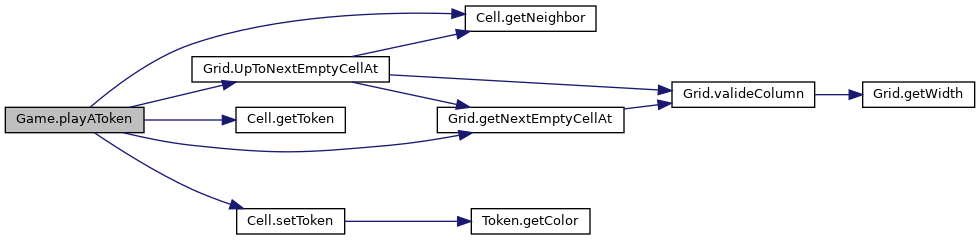
\includegraphics[width=.9\linewidth]{../doc/html/class_game_adc2797ea3355dc71d48a16af2f4b01b9_cgraph.png}
\caption{Graph d'appels de Game.play()}
\end{figure}

\item \texttt{isEnd: () -> ()}
\label{sec:orge0e3cb8}

Cette méthode teste si le jeu est terminée (victoire ou égalité), elle
actualise par effet de bord l'attribut: \texttt{this.end}.

\begin{enumerate}
\item \texttt{hasWin(): () -> boolean}
\label{sec:orgd926a0b}

Cette méthode teste si il y a un gagnant.

Pour cela elle appelle la méthode \texttt{check()} de la classe \hyperref[org0ebae20]{Cell} sur la
dernière cellule modifiée: càd la dernière cellules correspondant à
la dernière colonne jouée.\\

\item \texttt{isTie: () -> boolean}
\label{sec:org6216414}

Cette méthode teste l'égalité du jeu: elle retourne la comparaison
entre le nombre itération du jeu et le nombre de case disponible dans
la grille.

\begin{figure}[htbp]
\centering
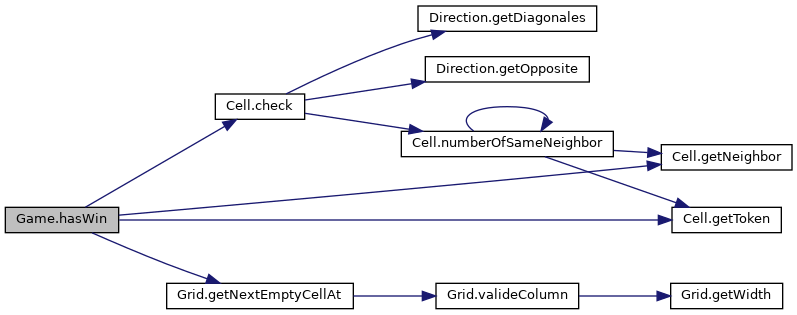
\includegraphics[width=.9\linewidth]{../doc/html/class_game_ac6f57b9a3185438aa0ca54d03dd5d3b5_cgraph.png}
\caption{Graph d'appels de Game.hasWin()}
\end{figure}

\begin{figure}[htbp]
\centering
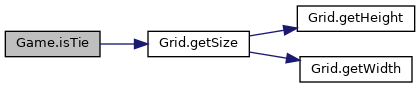
\includegraphics[width=7cm]{../doc/html/class_game_a019583b1c7288eb5eaf25dc13065c519_cgraph.png}
\caption{Graph d'appels de Game.isTie()}
\end{figure}
\end{enumerate}
\end{enumerate}

\subsection{Classe Save\label{orgc3d7ebb}}
\label{sec:org39e23c7}

Cette classe a été écrite pour être indépendant du jeu puissance 4, cette
classe comporte juste deux méthode, lire et écrire dans un fichier. 

\subsubsection{Attribut}
\label{sec:org5736d1b}

Cette classe comporte un seul attribut représentant le fichier par son
chemin d'accès représenté par une String.

\subsubsection{Méthodes}
\label{sec:org8f411e6}
\begin{enumerate}
\item \texttt{write: Object -> ()}
\label{sec:org23fbb1b}

Cette méthode écrit dans le fichier l'appelle à la méthode toString()
de l'objet en paramètre.\\

\item \texttt{read: () -> String}
\label{sec:org06084db}

Cette méthode lit dans le fichier et renvoie sa représentation sous la
forme d'une chaîne de caractères.
\end{enumerate}

\subsection{Enumérations}
\label{sec:org2320895}

Nous avons implémenté 3 énumérations dans notre logiciel.

\subsubsection{Entity\label{org0316ddb}}
\label{sec:orgb31bd54}

Cette énumération possède 2 attributs: \textbf{LOCAL}, \textbf{IA}. Elle définit la
nature du joueur: si c'est un joueur humain (\textbf{LOCAL}) ou un ordinateur
(\textbf{IA}). 

Elle possède une fonction qui retourne l'Entity correspondant à une
chaîne de caractères passées en paramètre: \texttt{of: String -> Entity}.

\subsubsection{Color\label{orgc449396}}
\label{sec:orga264443}

Cette enumération possède 3 attributs : RED, YELLOW, EMPTY
EMPTY désigne la couleur vide pour les cellules initialisées.

Elle possède quelques fonctions utiles comme :

\begin{itemize}
\item \texttt{ansiColorOf: String -> String} retourner les couleurs ansi suivant la
chaine de caractères passée en paramètre.
\begin{itemize}
\item \texttt{colorOf: String -> Color} retourner la couleur de type Color par une
\end{itemize}
chaine de caractère donnée en paramètre.
\end{itemize}

\subsubsection{Direction\label{org149a95e}}
\label{sec:orgd2ff209}

Cette énumération possède 4 attributs qui sont les directions des
cellules voisines à une cellule: \textbf{UP}, \textbf{DOWN}, \textbf{RIGHT}, \textbf{LEFT}.

Elle possède une fonction retournant les diagonales sous forme d'une
EnumMap:

\begin{itemize}
\item \texttt{of: () -> EnumMap<Direction, Direction>}. Les clés sont les
\end{itemize}
directions primaires et les valeurs une direction formant la
diagonale. La fonction est prévu pour assurer l'unicité des diagonales.

\section{Documentation\label{org29fdec9}}
\label{sec:org900457b}

La documentation est entièrement disponible dans le dossier \textbf{doc/}. La
documentation a été générer grâce à l'outil DOxyGen (1.9.3). Elle contient le
diagramme de classe de chaque classe du logiciel ainsi que les graphes
d'appels (Call \& Caller). 

La documentation est mise sous \textbf{HTML} et \textbf{\LaTeX{}}.

Le fichier \textbf{HTML} est disponible \href{/home/hozen/cur/projet-java/doc/html/index.html}{../doc/html/index.html}.

Le fichier \textbf{PDF} compilé à partir du \textbf{\LaTeX{}} est disponible
\href{/home/hozen/cur/projet-java/doc/latex/refman.pdf}{../doc/latex/refman.pdf}.

\section{Git\label{orgacd542c}}
\label{sec:orgce425cf}

Le projet est disponible et hébergé sur le \href{https://gitlab.isima.fr}{GitLab de l'ISIMA}

\newpage
\listoffigures
\end{document}
